\documentclass[12pt]{article}

% ---------- Layout ----------
\usepackage[a4paper, top=1.8cm, bottom=2.0cm, left=1.9cm, right=1.9cm]{geometry}
\usepackage{fontspec}
\setmainfont{Arial}
\usepackage{setspace}
\setstretch{1.0}

% ---------- Packages ----------
\usepackage{amsmath, amssymb, amsfonts}
\usepackage{graphicx}
\usepackage{booktabs}
\usepackage{float}
\usepackage{caption}
\usepackage{subcaption}
\usepackage{enumitem}
\usepackage{xcolor}
\usepackage{hyperref}
\usepackage{fancyhdr}
\usepackage{array}
\usepackage{tabularx}
\usepackage{multicol}

% ---------- Colors ----------
\definecolor{linkblue}{RGB}{0, 102, 204}
\definecolor{secgray}{RGB}{80, 80, 80}

% ---------- Header / Footer ----------
\pagestyle{fancy}
\fancyhf{}
\renewcommand{\headrulewidth}{0.4pt}
\fancyhead[L]{\small\textcolor{secgray}{S\&P 500 Market Direction}}
\fancyhead[R]{\small\textcolor{secgray}{\textsc{MLOps Report}}}
\fancyfoot[C]{\thepage}

% ---------- Section formatting ----------
\usepackage{titlesec}
\titleformat{\section}{\large\bfseries}{\thesection}{0.6em}{}
\titleformat{\subsection}{\normalsize\bfseries}{\thesubsection}{0.5em}{}
\titlespacing*{\section}{0pt}{8pt}{3pt}
\titlespacing*{\subsection}{0pt}{6pt}{2pt}

% ---------- Caption style ----------
\captionsetup{font=small, labelfont=bf, skip=3pt}

% ---------- Paragraph style ----------
\setlength{\parindent}{0pt}
\setlength{\parskip}{3.5pt}

% ---------- Hyperlinks ----------
\hypersetup{colorlinks=true, linkcolor=linkblue, citecolor=linkblue, urlcolor=linkblue}

% ---------- Graphics ----------
\graphicspath{{../data/08_reporting/plots/}{../data/08_reporting/shap/}}
\emergencystretch=1em

\newcommand{\boldparagraph}[1]{\textbf{#1}\hspace{5pt}}
\newcommand{\cmark}{\textcolor{green!55!black}{\checkmark}}

\begin{document}

% =====================================================================
% TITLE
% =====================================================================
\thispagestyle{empty}
\begin{center}
    \vspace*{-0.6cm}
    {\LARGE \textbf{S\&P 500 Market Direction}}\\[1pt]
    {\large \textbf{An End-to-End MLOps Pipeline (Proof of Concept)}}\\[5pt]
    {\small
    Miguel Ven\^ancio \quad Ant\'onio Varela \quad Maria Cruz \quad Carlos Amorim}\\[2pt]
    {\footnotesize NOVA Information Management School (NOVA IMS), 2025/2026 \;\textbullet\;
    \href{https://github.com/vehnie/sp500-mlops-pipeline}{github.com/vehnie/sp500-mlops-pipeline}}
\end{center}
\vspace{2pt}
\hrule height 0.5pt
\vspace{5pt}

% =====================================================================
% 1. MOTIVATION, OBJECTIVES, SUCCESS METRICS
% =====================================================================
\section{Data Choice, Objectives \& Success Metrics}

\boldparagraph{Why this data.} We use daily OHLCV history of the S\&P 500 index (Yahoo Finance, ticker \texttt{\^{}GSPC}, 2000--2026, 6{,}604 usable rows). The choice is deliberate for an \textit{MLOps} project rather than a pure modelling one: the data is free, clean, reliably available, and updates every trading day, so it realistically exercises ingestion, scheduling, and drift monitoring. It is also a genuine time series, which forces correct, leak-free engineering (chronological splits, time-aware validation and monitoring), and it represents a \textit{low-signal} problem, which is exactly where solid operational tooling earns its value: small pipeline mistakes can masquerade as ``performance'', so contracts and tracking are essential.

\boldparagraph{What we try to achieve.} The task is binary classification: predict whether the next trading day closes higher than today, $y_t = \mathbb{1}[\text{Close}_{t+1} > \text{Close}_t]$. The real objective, however, is to deliver a \textbf{production-grade ML lifecycle}: reproducible orchestration (Kedro), experiment tracking and a model registry (MLflow), data contracts (Great Expectations), drift monitoring (Evidently), explainability (SHAP), a served REST API (FastAPI + Docker), and automated tests (pytest). The model itself is intentionally simple so the engineering around it is the deliverable.

\boldparagraph{Success metrics.} We track success on two levels (Table~\ref{tab:success}). \textit{Model metrics} are Accuracy, Precision, Recall, F1, and ROC-AUC, with \textbf{ROC-AUC as the primary discrimination metric} since it is threshold-independent and robust to the mild class imbalance. \textit{System (MLOps) metrics} define what ``done'' means operationally and are, for this PoC, the more important bar.

\vspace{-3pt}
\begin{table}[H]
\centering
\small
\caption{Success criteria and final status.}
\label{tab:success}
\begin{tabularx}{\textwidth}{lXc}
\toprule
\textbf{Level} & \textbf{Criterion} & \textbf{Status} \\
\midrule
Model & ROC-AUC reported honestly on a leak-free chronological test set & \cmark\ 0.499 \\
Model & Champion beats challenger on the selection metrics (Acc/Recall/F1) & \cmark \\
System & One-command reproducible run (\texttt{kedro run}) from raw to predictions & \cmark \\
System & Data contracts pass at raw and feature layers & \cmark\ 19/19, 27/27 \\
System & Model tracked, versioned, and registered with lineage (MLflow) & \cmark \\
System & Drift monitor produces an actionable report & \cmark \\
System & Champion served behind a REST API + container & \cmark \\
System & Automated test suite green & \cmark\ 80 passed \\
\bottomrule
\end{tabularx}
\end{table}

% =====================================================================
% 2. SYSTEM ARCHITECTURE
% =====================================================================
\section{System Architecture \& Data Quality}

The system is a directed acyclic graph of \textbf{Kedro} pipelines, each a set of nodes with declared inputs/outputs registered in a central data catalog, so every artifact is traceable to the node that produced it. A single \texttt{kedro run} executes the default end-to-end workflow:

\vspace{-1pt}
\begin{center}
\footnotesize\texttt{data\_quality $\rightarrow$ data\_cleaning $\rightarrow$ data\_feat\_engineering $\rightarrow$ data\_split $\rightarrow$ model\_train $\rightarrow$ model\_train\_challenger $\rightarrow$ model\_predict $\rightarrow$ model\_predict\_challenger}
\end{center}
\vspace{-1pt}

Three further pipelines, \texttt{data\_\allowbreak expectations} (contracts), \texttt{model\_\allowbreak explainability} (SHAP), and \texttt{data\_\allowbreak drift} (Evidently), run on demand to generate the validation, interpretability, and monitoring artifacts. Table~\ref{tab:stack} maps each MLOps concern to its implementing tool. \textbf{Data quality} is enforced with Great Expectations at two checkpoints: a \textit{raw contract} (OHLCV schema/types, non-null prices, \texttt{High}$\geq$\texttt{Low}, positive volume, valid dates) and a \textit{feature contract} (all eight features finite, \texttt{rsi\_14}$\in[0,100]$, target $\in\{0,1\}$). Both pass fully in the final run (19/19 and 27/27), so a future data refresh that breaks an assumption fails loudly and early.

\begin{table}[H]
\centering\small
\caption{MLOps concerns and the components implementing them.}
\label{tab:stack}
\begin{tabularx}{\textwidth}{XX}
\toprule
Pipeline orchestration \& catalog \;\textemdash\; \textbf{Kedro} & Drift monitoring \;\textemdash\; \textbf{Evidently} \\
Experiment tracking \& registry \;\textemdash\; \textbf{MLflow} & Model serving (REST API) \;\textemdash\; \textbf{FastAPI + Uvicorn} \\
Data \& feature contracts \;\textemdash\; \textbf{Great Expectations} & Containerisation \;\textemdash\; \textbf{Docker / Compose} \\
Explainability \;\textemdash\; \textbf{SHAP} (\texttt{LinearExplainer}) & Automated testing \;\textemdash\; \textbf{pytest} (80 tests) \\
\bottomrule
\end{tabularx}
\end{table}

% =====================================================================
% 3. PROJECT PLANNING
% =====================================================================
\section{Project Planning (Agile Sprints)}

We organised the work as six one-week sprints with a Kanban board of pipeline-sized tasks. Each sprint produced a runnable increment: a new Kedro pipeline plus its tests and catalog entries were the ``definition of done''. This kept the system end-to-end runnable at every stage and let monitoring/serving be added without touching the core training path.

\vspace{-3pt}
\begin{table}[H]
\centering
\small
\caption{Sprint plan. Each sprint delivers one or more registered Kedro pipelines.}
\label{tab:sprints}
\begin{tabularx}{\textwidth}{p{1.3cm}p{4.6cm}X}
\toprule
\textbf{Sprint} & \textbf{Goal} & \textbf{Key deliverables} \\
\midrule
S0 & Setup \& exploration & Repo, Kedro scaffold, \texttt{data\_ingestion}, EDA notebooks \\
S1 & Data foundation & \texttt{data\_cleaning}, \texttt{data\_feat\_engineering}, \texttt{data\_split} (chronological 70/15/15), target definition \\
S2 & Data quality & \texttt{data\_quality} + \texttt{data\_expectations} (Great Expectations contracts) \\
S3 & Modelling \& tracking & \texttt{model\_train} (LR champion), \texttt{model\_train\_challenger} (RF), MLflow tracking + registry \\
S4 & Evaluation \& explainability & \texttt{model\_predict(\_challenger)}, reporting plots, \texttt{model\_explainability} (SHAP) \\
S5 & Monitoring, serving \& hardening & \texttt{data\_drift} (Evidently), FastAPI + Docker, Streamlit, pytest suite, docs/report \\
\bottomrule
\end{tabularx}
\end{table}

% =====================================================================
% 3. RESULTS
% =====================================================================
\section{Results: Exploration \& Modelling}

\boldparagraph{Data exploration.} The index level is strongly trending and \textit{non-stationary}, while daily returns are stationary around zero with clustered volatility (Figure~\ref{fig:eda}). The target is mildly skewed toward up-days ($\approx 53\%$), consistent with long-run equity drift. From the price and volume we engineer eight leak-free features (all using information up to day $t$): \texttt{simple\_return}, \texttt{log\_return}, \texttt{sma\_10}, \texttt{sma\_20}, \texttt{sma\_ratio\_10}, \texttt{rsi\_14}, \texttt{volatility\_10}, \texttt{volume\_change}. The set is kept small so every feature stays inspectable.

\begin{figure}[H]
    \centering
    \begin{subfigure}[t]{0.32\textwidth}\centering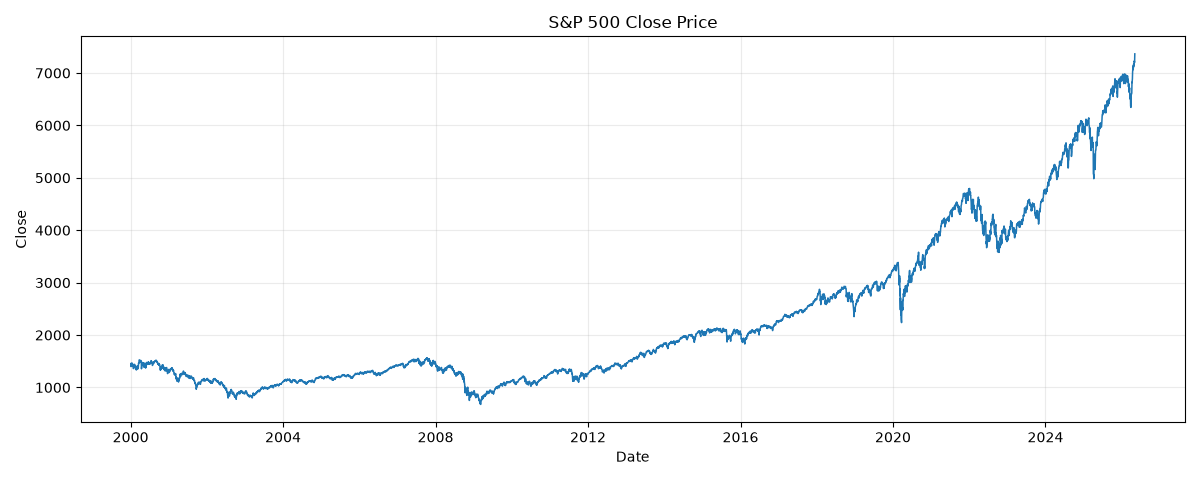
\includegraphics[width=\textwidth]{sp500_close_price.png}\caption{Close price (non-stationary).}\end{subfigure}\hfill
    \begin{subfigure}[t]{0.32\textwidth}\centering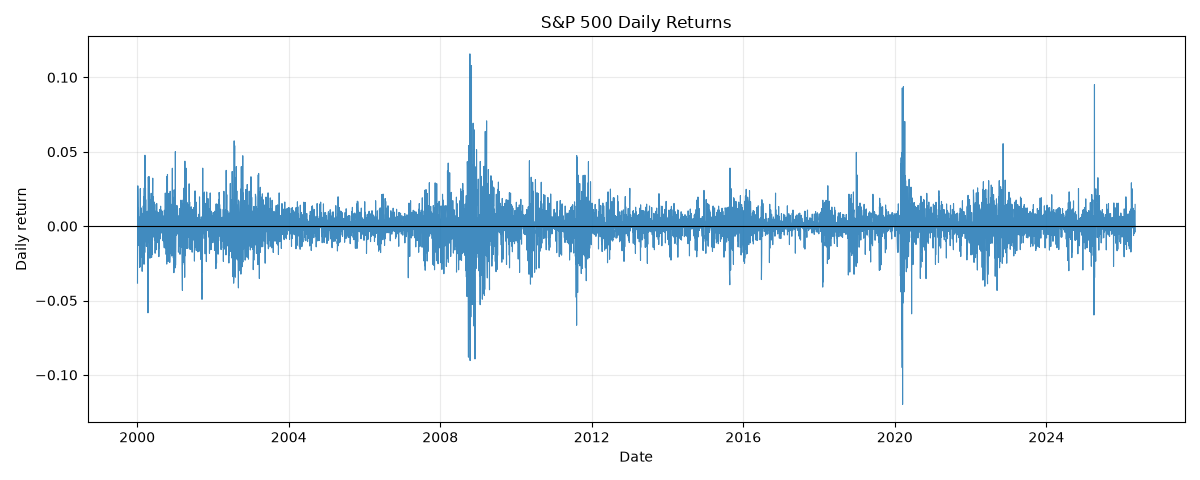
\includegraphics[width=\textwidth]{sp500_daily_returns.png}\caption{Daily returns (stationary).}\end{subfigure}\hfill
    \begin{subfigure}[t]{0.32\textwidth}\centering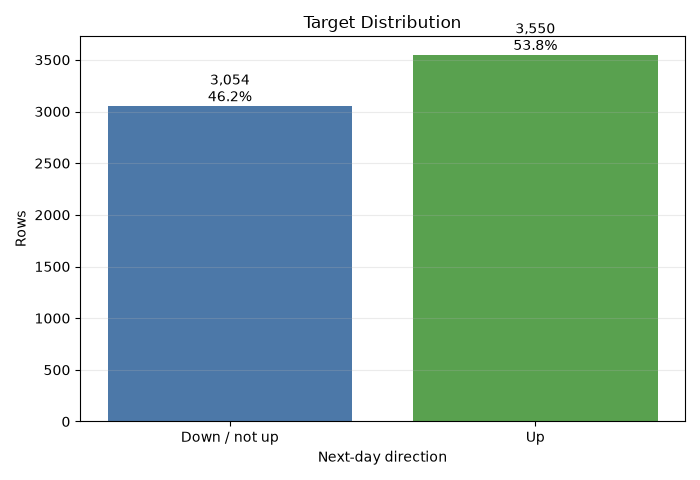
\includegraphics[width=\textwidth]{sp500_target_distribution.png}\caption{Target balance ($\approx$53\% up).}\end{subfigure}
    \caption{Exploratory analysis. Trending levels vs.\ stationary returns directly motivate the drift findings below.}
    \label{fig:eda}
\end{figure}

\boldparagraph{Modelling.} We compare a \textbf{champion} (\texttt{StandardScaler} + Logistic Regression) against a \textbf{challenger} (Random Forest, 300 trees, depth 8, regularised), both trained and evaluated under the identical chronological split with MLflow tracking. Results on the held-out test block (992 future rows) are in Table~\ref{tab:results}.

\vspace{-3pt}
\begin{table}[H]
\centering\small
\caption{Test-set performance. Champion selected on Accuracy/Recall/F1; both show near-random ROC-AUC.}
\label{tab:results}
\begin{tabular}{lccccc}
\toprule
\textbf{Model} & \textbf{Accuracy} & \textbf{Precision} & \textbf{Recall} & \textbf{F1} & \textbf{ROC-AUC} \\
\midrule
\textbf{Logistic Regression} (champion) & \textbf{0.536} & 0.542 & \textbf{0.922} & \textbf{0.683} & 0.499 \\
Random Forest (challenger) & 0.503 & \textbf{0.547} & 0.473 & 0.507 & \textbf{0.502} \\
\bottomrule
\end{tabular}
\end{table}

\begin{figure}[H]
    \centering
    \begin{subfigure}[t]{0.30\textwidth}\centering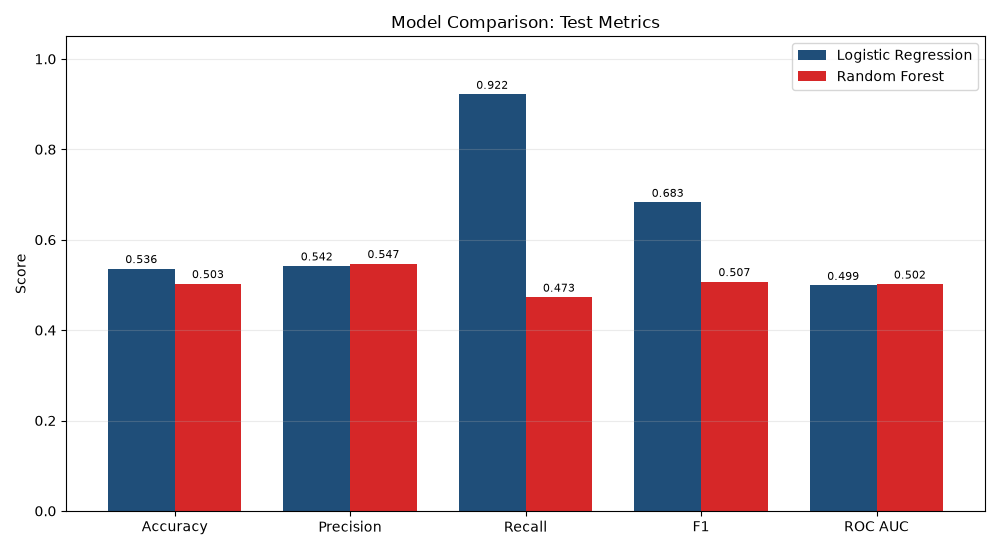
\includegraphics[width=\textwidth]{model_comparison.png}\caption{Champion vs.\ challenger.}\end{subfigure}\hfill
    \begin{subfigure}[t]{0.30\textwidth}\centering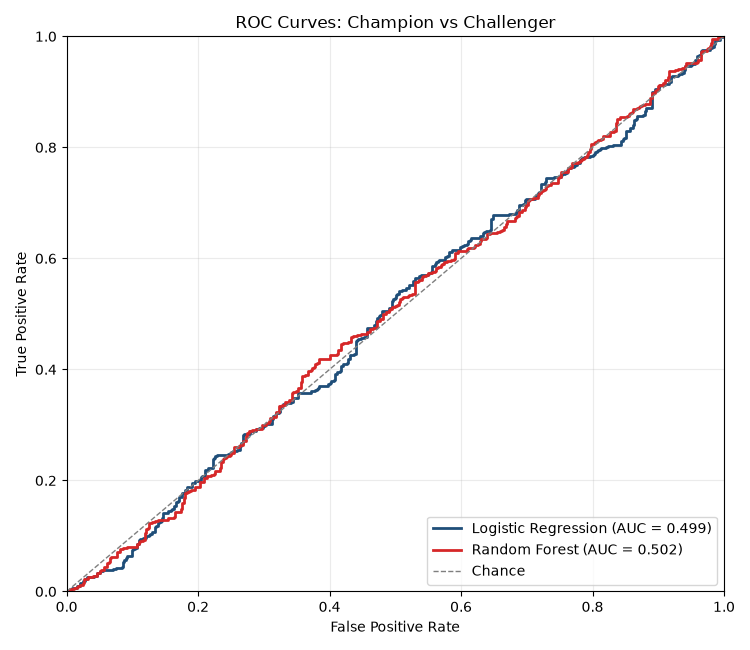
\includegraphics[width=\textwidth]{roc_curves.png}\caption{ROC curves ($\approx$ diagonal).}\end{subfigure}\hfill
    \begin{subfigure}[t]{0.36\textwidth}\centering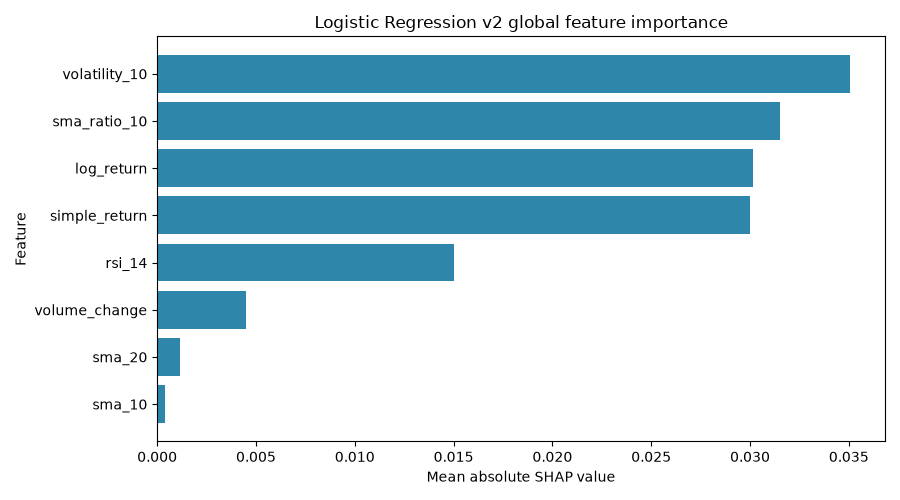
\includegraphics[width=\textwidth]{logistic_regression_v2_feature_importance_bar.png}\caption{SHAP feature importance.}\end{subfigure}
    \caption{(a) The champion leads on Accuracy/Recall/F1. (b) Both ROC curves hug the chance diagonal (AUC $\approx0.50$). (c) SHAP ranks \texttt{volatility\_10} and \texttt{sma\_ratio\_10} highest, but all magnitudes are small.}
    \label{fig:eval}
\end{figure}

The behavioural difference is clear in Figure~\ref{fig:eval2}: the champion concentrates predictions on the up-class (high recall, many false positives), while the challenger spreads errors more evenly; both predicted-probability distributions cluster tightly around 0.5, the visual signature of an appropriately uncertain model.

\begin{figure}[H]
    \centering
    \begin{subfigure}[t]{0.40\textwidth}\centering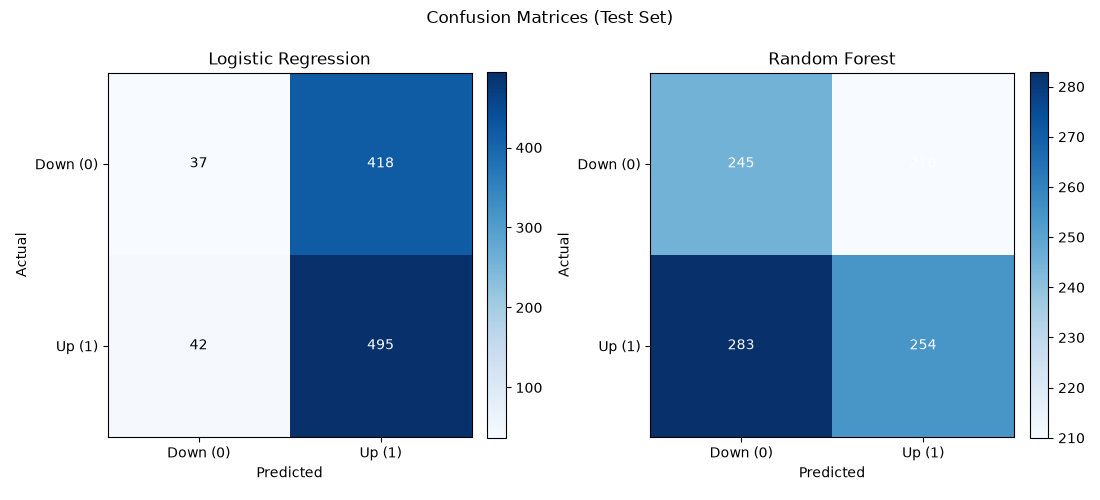
\includegraphics[width=\textwidth]{confusion_matrices.png}\caption{Confusion matrices.}\end{subfigure}\hfill
    \begin{subfigure}[t]{0.40\textwidth}\centering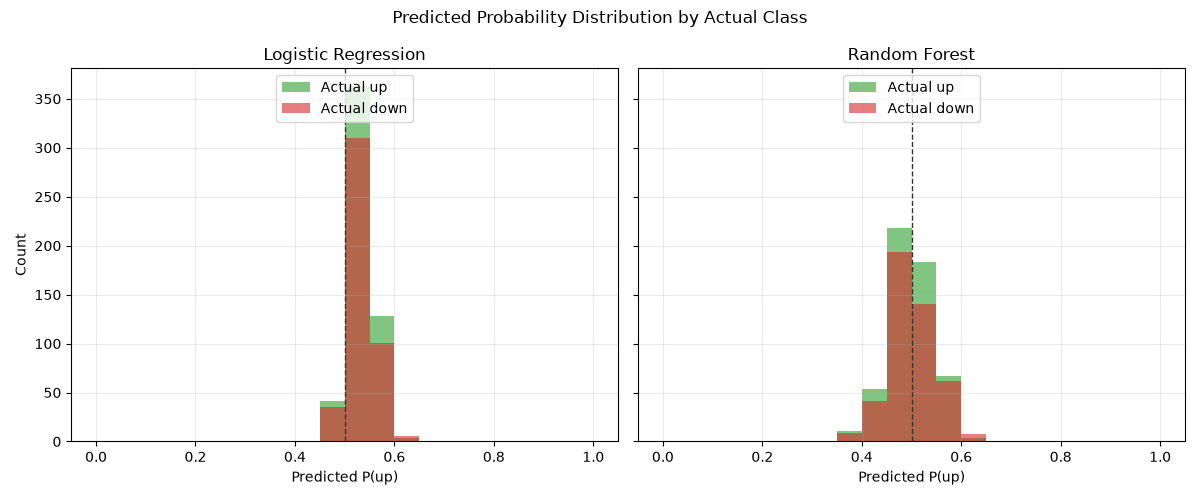
\includegraphics[width=\textwidth]{probability_distribution.png}\caption{Predicted-probability distributions.}\end{subfigure}\hfill
    \begin{subfigure}[t]{0.18\textwidth}\centering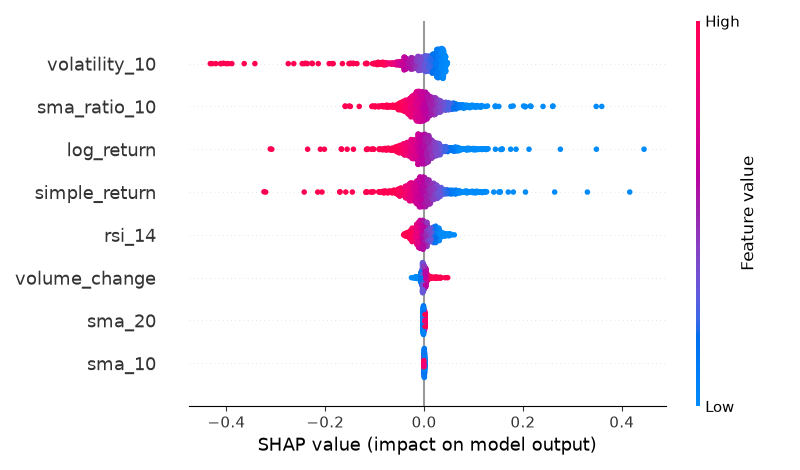
\includegraphics[width=\textwidth]{logistic_regression_v2_summary_plot.png}\caption{SHAP beeswarm.}\end{subfigure}
    \caption{(a) The champion predicts mostly ``up''; (b) probabilities concentrate near 0.5; (c) per-observation SHAP values stay small and centred on the base value.}
    \label{fig:eval2}
\end{figure}

\boldparagraph{Explainability.} SHAP (exact \texttt{LinearExplainer} on the champion, Figures~\ref{fig:eval}c and~\ref{fig:eval2}c) shows the model leans most on recent risk (\texttt{volatility\_10}, mean$|$SHAP$|=0.035$) and distance from trend (\texttt{sma\_ratio\_10}, $0.032$), with returns close behind, all intuitive for a short-horizon signal. Crucially, every attribution is \textit{small}, matching the headline finding: \textbf{ROC-AUC $\approx 0.50$ means neither model ranks up-days above down-days better than chance.} The champion's high recall (0.922) simply reflects it predicting ``up'' most days, exploiting the class prior rather than real discrimination.

\boldparagraph{Drift \& conclusion.} The Evidently monitor compares the oldest 70\% (reference, 4{,}622 rows) against the newest 30\% (current, 1{,}982 rows) with a normalised Wasserstein distance (threshold 0.1) and flags \textbf{dataset-level drift}: 4 of 8 features drift (Table~\ref{tab:drift}), driven almost entirely by the non-stationary moving averages \texttt{sma\_10}/\texttt{sma\_20} (scores $>6$), while the stationary return features do not. This is exactly the expected behaviour and pinpoints the features a production system should reformulate. Overall, the leak-free split, passing contracts, small SHAP magnitudes, and interpretable drift together confirm that the weak result is \textit{real}, not an artifact, which is precisely what trustworthy MLOps tooling should reveal.

\vspace{-3pt}
\begin{table}[H]
\centering\small
\caption{Evidently drift report (Wasserstein distance, threshold 0.1). Dataset drift flagged: 4/8 features, share 0.50.}
\label{tab:drift}
\begin{tabular}{lcc|lcc}
\toprule
\textbf{Feature} & \textbf{Score} & \textbf{Drift} & \textbf{Feature} & \textbf{Score} & \textbf{Drift} \\
\midrule
\texttt{sma\_20} & 6.154 & \textbf{Yes} & \texttt{volume\_change} & 0.097 & No \\
\texttt{sma\_10} & 6.145 & \textbf{Yes} & \texttt{volatility\_10} & 0.071 & No \\
\texttt{rsi\_14} & 0.173 & \textbf{Yes} & \texttt{simple\_return} & 0.057 & No \\
\texttt{sma\_ratio\_10} & 0.105 & \textbf{Yes} & \texttt{log\_return} & 0.057 & No \\
\bottomrule
\end{tabular}
\end{table}

% =====================================================================
% SERVING & REPRODUCIBILITY
% =====================================================================
\section{Serving, Tracking \& Reproducibility}

Every training run logs its parameters, metrics, tags (e.g.\ \texttt{split\_strategy = chronological\_70\_15\_15}), feature list, model signature, and serialised artifact to \textbf{MLflow}. The champion is registered as \texttt{sp500\_direction\_model} and exposed to serving by the registry alias \texttt{candidate\_champion}, so a newly promoted model is picked up without code changes. The \textbf{FastAPI} service exposes \texttt{GET /health}, \texttt{GET /model-info}, and \texttt{POST /predict} (Pydantic-validated eight-feature input $\rightarrow$ class + probability), and is packaged as the Docker image \texttt{sp500-direction-api}. Reproducibility is structural: all datasets live in the Kedro catalog, all parameters in versioned \texttt{conf/} files, random states fixed to 42, and an 80-test \textbf{pytest} suite plus the data contracts give two independent safety nets (tests catch code regressions, contracts catch data regressions).

% =====================================================================
% 5. PRODUCTION
% =====================================================================
\section{From Proof of Concept to Production}

This PoC runs locally: Pandas in-memory, a local MLflow server with a SQLite backend and file artifacts, a file-based feature layer, and \texttt{yfinance} for data. The technology choices are deliberately production-aligned, so the path to deployment is incremental rather than a rewrite. \textbf{Advantages of the stack:} Kedro gives modular, catalog-driven pipelines that map cleanly onto an orchestrator (Airflow/Kubeflow); MLflow already provides model lineage, versioning, and a registry the API loads by alias; Great Expectations and Evidently make data quality and drift first-class and CI-friendly; FastAPI + Docker yield a portable, horizontally scalable service; pytest plus the data contracts give two independent safety nets. Table~\ref{tab:risks} lists the main PoC limitations with proposed, effort-scoped mitigations.

\vspace{-3pt}
\begin{table}[H]
\centering\small
\caption{Production risks and proposed mitigations (effort as additional sprints).}
\label{tab:risks}
\begin{tabularx}{\textwidth}{p{3.5cm}Xc}
\toprule
\textbf{Risk / limitation} & \textbf{Proposed mitigation} & \textbf{Effort} \\
\midrule
Pandas is single-node; will not scale to large/intraday data & Port feature/cleaning nodes to Spark (Kedro keeps the same node interface) & +3 wk \\
Local MLflow (SQLite + file store) is not multi-user or durable & Managed tracking server + cloud artifact store (e.g.\ S3/Postgres backend) & +1 wk \\
File-based feature layer, no online serving & Adopt a feature store (Feast/Hopsworks) for train/serve parity & +2 wk \\
\texttt{yfinance} is an unofficial, rate-limited source & Scheduled ingestion via a licensed market-data vendor + retries/back-off & +1 wk \\
Drift is detected but retraining is manual & CI/CD pipeline with drift-triggered, automated retraining \& promotion gates & +2 wk \\
Weak signal (ROC-AUC $\approx$ 0.50) & Add alternative data (macro, sentiment, cross-asset), calibrate, walk-forward backtest & +3 wk \\
API has no auth / observability & Add auth, rate limiting, logging, and metrics (Prometheus/Grafana) & +1 wk \\
\bottomrule
\end{tabularx}
\end{table}

% =====================================================================
% 5. PACKAGES
% =====================================================================
\section{Packages and Versions}

Developed on \textbf{Python 3.11.9}. Core dependencies (pinned versions used for the final run):

\vspace{-2pt}
\begin{multicols}{2}
\small
\begin{itemize}[leftmargin=1.1em, itemsep=0pt, topsep=1pt]
\item \texttt{kedro==1.4.0}
\item \texttt{kedro-datasets==9.4.0}
\item \texttt{yfinance==1.4.1}
\item \texttt{pandas==2.3.3}
\item \texttt{numpy==2.4.6}
\item \texttt{scikit-learn==1.9.0}
\item \texttt{matplotlib==3.11.0}
\item \texttt{mlflow==3.14.0}
\item \texttt{shap==0.51.0}
\item \texttt{fastapi==0.138.0}
\item \texttt{uvicorn==0.49.0}
\item \texttt{pydantic==2.13.4}
\item \texttt{great\_expectations==1.18.1}
\item \texttt{evidently==0.7.21}
\item \texttt{streamlit==1.58.0}
\item \texttt{python-dotenv==1.2.2}
\item \texttt{pytest==9.1.1}
\end{itemize}
\end{multicols}

% =====================================================================
% REFERENCES
% =====================================================================
\vspace{2pt}
\hrule height 0.3pt
\vspace{4pt}
\renewcommand{\refname}{References}
\begin{thebibliography}{1}
\small
\bibitem{yahoofinance}
Yahoo Finance. S\&P 500 index (\texttt{\^{}GSPC}) historical data.
\url{https://finance.yahoo.com/quote/\%5EGSPC/chart/}
\end{thebibliography}

\end{document}
